\section{Time plots}

\begin{figure}
\centering
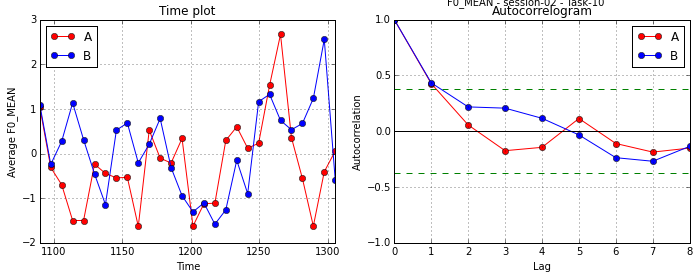
\includegraphics[width=15cm]{images/time_plot_with_autocorrelation.png}
\caption{Time-plot producido por TAMA, junto a su autocorrelación \label{time_plot}}

\end{figure}

Usando la técnica descripta, generamos dos series de tiempo para cada tarea. Como antes mencionamos, la ventana elegida es de $16''$ con un step de $8''$ lo cual da un overlap del 50\%.

Dada una ventana, puede ocurrir que alguno de los interlocutores no haya hablado, o su interacción haya sido demasiado breve como para medir sus variables a/p. En ese caso, y a diferencia de \cite{KOU2008}, construimos las series sin ese punto, y sin interpolarlo tampoco. (¿por qué no estamos interpolando en vez de )

De estas tareas, sólo nos quedamos con aquellas que tengan al menos 5 puntos definidos para cada serie, de manera que tenga sentido poder calcular la correlación cruzada más adelante (¿podemos justificar un poco más ésto?).